\documentclass[a4paper, 11pt]{article}

% --- ENCODING ---
\usepackage[utf8]{inputenc}
\usepackage[T1]{fontenc}
\usepackage[italian]{babel}

% --- FONT E MICRO-TIPOGRAFIA ---
\usepackage{lmodern}
\usepackage{microtype}
\tolerance=1000
\emergencystretch=2em

% --- MATEMATICA ---
\usepackage{amsmath}
\usepackage{amssymb}
\usepackage{amsthm}

% --- GRAFI E GRAFICA ---
\usepackage{tikz}
\usetikzlibrary{graphs, trees, positioning, arrows.meta, shapes, calc, backgrounds}

% --- ALGORITMI ---
\usepackage[ruled, vlined, linesnumbered, onelanguage]{algorithm2e}

% --- FIGURE E TABELLE ---
\usepackage{graphicx}
\usepackage{float}
\usepackage{caption}
\usepackage{subcaption}
\usepackage{booktabs}
\usepackage{array}
\usepackage{colortbl}
\usepackage{tikz}
\usepackage{pgfplots}
\pgfplotsset{compat=1.18}  


% --- LAYOUT E UTILITÀ ---
\usepackage{geometry}
\usepackage{xcolor}
\usepackage{xspace}
\usepackage{listings}
\usepackage{setspace}
\usepackage{fancyhdr}
\usepackage{emptypage}
\usepackage{titlesec}
\usepackage{tocloft}

% --- HYPERREF SEMPRE PER ULTIMO ---
\usepackage[hidelinks, plainpages=false, pdfpagelabels]{hyperref}

% --- PROFONDITÀ INDICE ---
\setcounter{tocdepth}{3}
\setcounter{secnumdepth}{3}

% --- COLORI ---
\definecolor{primary}{RGB}{0, 25, 127}
\definecolor{codegreen}{RGB}{0, 120, 0}
\definecolor{codegray}{RGB}{120, 120, 120}
\definecolor{codered}{RGB}{160, 0, 0}
\definecolor{codebg}{RGB}{248, 248, 248}

% --- GEOMETRIA ---
\geometry{
	a4paper,
	top=3cm, bottom=3cm,
	left=2.5cm, right=2.5cm,
	headheight=24.02pt
}

% --- INTERLINEA ---
\onehalfspacing
\setlength{\parindent}{0pt}
\setlength{\parskip}{0.5em}

% --- STILE TITOLI ---
\titleformat{\section}
{\Large\bfseries\color{primary}}
{\thesection.}{0.5em}{}
[\color{primary}\titlerule]

\titleformat{\subsection}
{\large\bfseries\color{primary}}
{\thesubsection}{0.5em}{}

\titleformat{\subsubsection}
{\normalsize\bfseries\color{primary}}
{\thesubsubsection}{0.5em}{}

\titlespacing{\section}{0pt}{2ex}{1ex}
\titlespacing{\subsection}{0pt}{1.5ex}{0.5ex}
\titlespacing{\subsubsection}{0pt}{1ex}{0.3ex}

% --- INTESTAZIONI ---
\pagestyle{fancy}
\fancyhf{}
\fancyhead[L]{\small\color{primary}\rightmark}
\fancyfoot[C]{\small\thepage}
\renewcommand{\headrulewidth}{0.4pt}
\makeatletter
\renewcommand{\headrule}{%
	\hbox to\headwidth{\color{primary}\leaders\hrule height\headrulewidth\hfill}}
\makeatother

% --- STILE INDICE ---
\renewcommand{\cftsecfont}{\bfseries\color{primary}}
\renewcommand{\cftsecpagefont}{\bfseries\color{primary}}
\renewcommand{\cftsubsecfont}{\color{primary}}
\renewcommand{\cftsubsecpagefont}{\color{primary}}
\renewcommand{\cftsubsubsecfont}{\color{primary}}
\renewcommand{\cftsubsubsecpagefont}{\color{primary}}

% --- TEOREMI ---
\newtheorem{teorema}{Teorema}[section]
\newtheorem{lemma}[teorema]{Lemma}
\newtheorem{corollario}[teorema]{Corollario}
\theoremstyle{definition}
\newtheorem{definizione}{Definizione}[section]
\newtheorem{nozione}{Nozione}[section]
\theoremstyle{remark}
\newtheorem{osservazione}{Osservazione}
\theoremstyle{remark}
\usepackage{tcolorbox}
\tcbuselibrary{theorems}
\newenvironment{nota}{%
	\begin{tcolorbox}[
		colback=codebg,
		colframe=primary,
		fonttitle=\bfseries,
		title=Nota,
		left=6pt, right=6pt, top=4pt, bottom=4pt
		]
	}{%
	\end{tcolorbox}
}

% --- KwAnd per algorithm2e ---
\SetKw{KwAnd}{and}

% --- LISTINGS ---
\lstset{
	language=Java,
	basicstyle=\ttfamily\small\color{black},
	keywordstyle=\color{primary}\bfseries,
	commentstyle=\color{codegreen}\itshape,
	stringstyle=\color{codered},
	numberstyle=\tiny\color{codegray},
	numbers=left,
	frame=single,
	rulecolor=\color{primary},
	backgroundcolor=\color{codebg},
	breaklines=true,
	breakatwhitespace=false,
	captionpos=b,
	showstringspaces=false,
	tabsize=4
}

% --- CAPTION ---
\captionsetup{font=small, labelfont={bf, color=primary}, labelsep=period}

% ================================================================
\begin{document}
	\pagenumbering{gobble}
	% --- FRONTESPIZIO ---
	\begin{titlepage}
		\centering
		\vspace*{3cm}
		{\large\scshape\color{primary} Università degli Studi di Verona}\\[0.3cm]
		{\large\color{black} Corso di Laurea in Bioinformatica}\\[0.2cm]
		\textcolor{primary}{\rule{\textwidth}{0.4pt}}\\[1.5cm]
		{\Huge\bfseries\color{primary} Algoritmi per Bioinformatica}\\[0.5cm]
		{\LARGE\color{black} e Laboratorio di Programmazione II}\\[2cm]
		\vfill
		{\large\color{black} I seguenti appunti sono preparati tramite i lucidi del professore e il libro di riferimento}
		
		{\large\color{black}} Per la parte di laboratorio il professore prende gli esercizi da:
		\url{https://leetcode.com/problemset/algorithms/}
		\textcolor{primary}{\rule{\textwidth}{0.4pt}}\\[0.5cm]
		{\large\color{black} Anno Accademico 2025/2026}
		
		
	\end{titlepage}
	\clearpage
	\pagenumbering{arabic}
	\tableofcontents
	\clearpage
	% ================================================================
	\section{Fondamenti}
		\subsection{Introduzione al corso}
			
			\subsubsection{Requisiti}
				\begin{itemize}
					\item Fondamenti di matematica discreta e grafi
					\item Calcolo delle probabilità
					\item Basi di C $\to$ si studia Java (Classi e Oggetti)\footnote{Java è il male}
					\item Le procedure ricorsive sono come l'Ave Maria (STUDIA: c'è nell'esame)
				\end{itemize}
			
			\subsubsection{Programma del corso}
				\begin{itemize}
					\item Divide et Impera
					\item Programmazione dinamica
					\item Algoritmi Greedy
					\item Grafi $\to$ Nodi e archi
				\end{itemize}
			
			\subsubsection{Struttura del modulo}
				48 ore di lezione: 4 ore a settimana + 9 ore di studio personale.\footnote{Sì, lo so, è una noia, ma serve.}
				Non usare ChatGPT o altri strumenti simili.
				
				I lucidi non bastano (purtroppo).
				
				Se proprio devi, usa \textbf{Anthropic CLAUDE}.
			
			\subsubsection{Modalità di esame}
				\begin{itemize}
					\item \textbf{Prima parte:} 15 domande a risposta multipla
					(almeno 4 su codice Java -- CODE RUNNER)
					\item \textbf{Seconda parte:} Progettare una soluzione algoritmica
					\item \textbf{Se va male:} Può fare orale se ha dubbi (Ave o Maria\dots)
				\end{itemize}
		
		% ================================================================
		\subsection{Il ruolo degli algoritmi nell'informatica}
		
			\subsubsection{Cos'è un algoritmo?}
			
				\begin{definizione}[Algoritmo]
					Procedura di calcolo ben definita: dato un input (anche nullo), produce un output
					in tempo finito.
				\end{definizione}
				
				\begin{definizione}[Problema computazionale]
					Relazione input/output desiderata. L'algoritmo specifica \textit{come} ottenerla.
				\end{definizione}
				
				\begin{definizione}[Algoritmo corretto]
					Termina producendo il risultato corretto per ogni istanza valida.
				\end{definizione}
				
				\begin{osservazione}
					Non sempre esiste un algoritmo: il problema della fermata è indecidibile.
				\end{osservazione}
		
		
		\subsection{Esempio di algoritmo ricorsivo}
			
			\begin{nota}
				Le convenzioni usate per il pseudocodice sono a pag. 19 del [CLRS].
			\end{nota}
				
			\begin{algorithm}[H]
				\caption{FibonacciR}
				\KwIn{$n \geq 0$}
				\KwOut{$F_n$}
				\If{$n = 0$}{\Return $0$\;}
				\If{$n = 1$}{\Return $1$\;}
				\Return FibonacciR($n-1$) + FibonacciR($n-2$)\;
			\end{algorithm}
			
			L’algoritmo è corretto? \textbf{Sì!}
			
			Per ogni input valido, termina? \textbf{Sì, assumendo che input sia sempre un intero n  $\geq$ 0}
			
			Se sì, calcola il valore giusto? \textbf{Sì, perché l’algoritmo codifica la definizione ricorsiva.}
			
			Quanto \textbf{tempo} richiede per terminare?
			
			\begin{figure}[H]
				\centering
				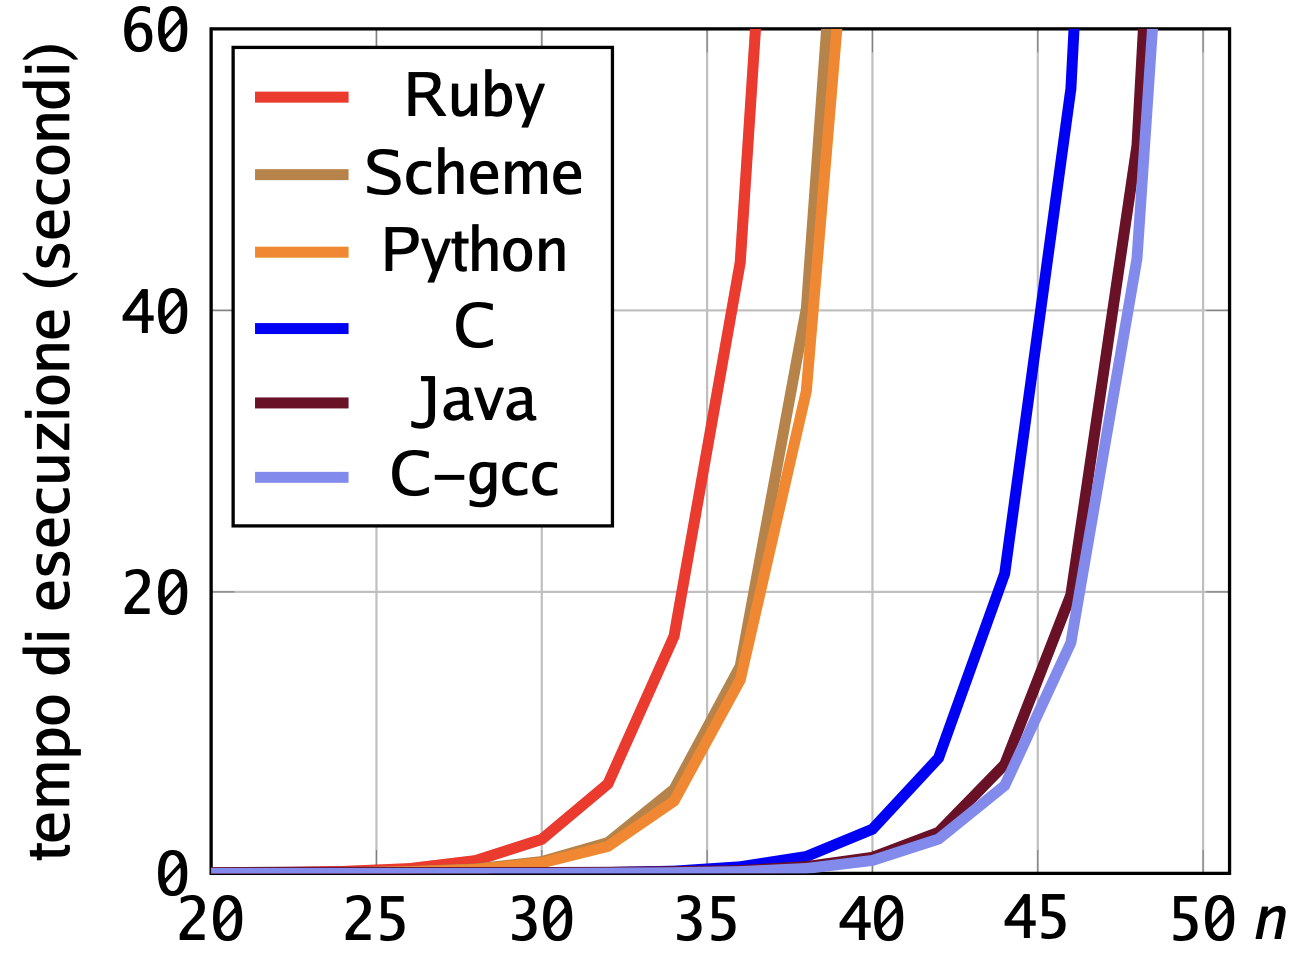
\includegraphics[width=0.5\textwidth]{Immagini/FibonacciT.png}
				\caption{Tempo computazionale dell'algoritmo \texttt{FibonacciR}}
				\label{fig:fibonacci-tempo}
				Come mostrato in Figura~\ref{fig:fibonacci-tempo}, il tempo cresce esponenzialmente.
				
			\end{figure}
			
			\newpage
				\subsubsection*{Calcolo della complessità computazionale}
			\begin{definizione}[Efficienza]
				Risorse (tempo e spazio) richieste in funzione della dimensione $n$ dell'input.
			\end{definizione}
			
			\begin{definizione}[Algoritmo vs.\ Implementazione]
				L'algoritmo è un concetto \textbf{astratto} ($\neq$ implementazione):
				descrive \textit{come} risolvere un problema indipendentemente dal linguaggio.
				L'implementazione è un \textbf{programma concreto}, ovvero la traduzione
				dell'algoritmo in un linguaggio comprensibile dalla \[
				T(n) = \begin{cases}
				mac & \text{se } condizione \\
				caso_ricorsivo & \text{altrimenti}
					\end{cases}
						\]
							china.
			\end{definizione}
			
			\begin{nozione}[Algoritmo efficiente]
				Andiamo a cercare l'algoritmo efficiente:
				\begin{itemize}
					\item \textbf{Efficiente:} usa poche risorse
					\item \textbf{Risorse:} tempo e spazio richiesti dall'algoritmo
					per produrre l'output
				\end{itemize}
			\end{nozione}
			
			\begin{teorema}[Algoritmo vs.\ hardware]
				Con $n = 10^7$ interi da ordinare:
				\begin{align*}
					t_A &= \frac{2(10^7)^2}{10^{10}} \approx 5.5\ \text{ore}
					\quad\text{(InsSort, } 10^9 \text{ istr/s)} \\
					t_B &= \frac{50 \cdot 10^7 \log_2 10^7}{10^6} \approx 20\ \text{min}
					\quad\text{(MergeSort, } 10^6 \text{ istr/s)}
				\end{align*}
				L'algoritmo migliore batte l'hardware più veloce.
			\end{teorema}
			
			\textbf{Possiamo fare meglio?}
			
			\subsubsection*{Ottimizzazione: FibonacciI }
			\begin{algorithm}[H]
				\caption{FibonacciI}
				\KwIn{Intero positivo $n$}
				\KwOut{Il valore $F_n$}
				\If{$n = 0$}{\Return $0$\;}
				\If{$n = 1$}{\Return $1$\;}
				$\mathit{pprev} = 0$\;
				$\mathit{prev} = 1$\;
				\For{$i = 2$ \KwTo $n$}{
					$f = \mathit{prev} + \mathit{pprev}$\;
					$\mathit{pprev} = \mathit{prev}$\;
					$\mathit{prev} = f$\;
				}
				\Return $f$\;
			\end{algorithm}
			
			La sua complessità soddisfa la ricorrenza:
			\[
			T(0) = 2, \quad T(1) = 3, \quad T(n) = T(n-1) + T(n-2) + 8
			\]
			
			Il $+8$ è dato da: 2 \texttt{if} + 2 calcoli parametri + 2 chiamate + 1 somma + 1 \texttt{return}.
			Da questa ricorrenza segue $T(n) > F_n$, e per $n \geq 7$:
			\[
			F_n > 2F_{n-2} > 2^2 F_{n-4} > \cdots > 2^{n/2}
			\]
			
			Quindi la crescita è \textbf{esponenziale}:
			\[
			T(n) > \left(\sqrt{2}\right)^n \approx (1.4)^n
			\]
			
			Una stima più precisa è data dalla \textbf{Formula di Binet}:
			\[
			T(n) \geq \frac{\varphi^n - (-\varphi)^{-n}}{\sqrt{5}}, \qquad \varphi = \frac{1+\sqrt{5}}{2} \approx 1.62
			\]
			
			L'algoritmo iterativo evita il ricalcolo sommando i valori dal più piccolo al più grande.
			La complessità è:
			\[
			T(0) = 2, \quad T(1) = 3, \quad T(n) = 4 + 2n + 4(n-1) + 1 = 6n + 1
			\]
			
			La crescita è \textbf{lineare in $n$}.
		
		
			\begin{center}
				\begin{tabular}{lll}
					\toprule
					Algoritmo & Complessità & $n=50$ \\
					\midrule
					Ricorsivo & $(1.4)^n$   & minuti \\
					Iterativo & $\Theta(n)$ & istantaneo \\
					\bottomrule
				\end{tabular}
			\end{center}
			
			\noindent\textbf{Modello RAM:} ogni operazione elementare ha costo $1$;
			parola di memoria a dimensione fissa.
			
		\subsection{Esempi di problemi computazionali da risolvere in aula}
			\subsubsection*{Iindici dei due numeri che sommati danno N}
				\textbf{Problema:} Data una matrice di interi \texttt{nums} e un intero \texttt{target}, restituisci gli indici dei due numeri tali che la loro somma sia uguale a \texttt{target}. Puoi assumere che ogni input abbia esattamente una soluzione, e non puoi usare lo stesso elemento due volte. Puoi restituire la risposta in qualsiasi ordine.
				
				\begin{algorithm}[H]
					\caption{twoSum (Brute Force)}
					\KwIn{\texttt{nums[0\ldots n-1]}, \texttt{target}}
					\KwOut{\{i, j\} tali che \texttt{nums[i] + nums[j] = target}, $i \neq j$}
					\For{$i = 0$ \KwTo $n-2$}{
						\For{$j = i+1$ \KwTo $n-1$}{
							\If{\texttt{nums[i] + nums[j] == target}}{
								\KwRet $\{i, j\}$\;
							}
						}
					}
				\end{algorithm}
				
				\noindent\textbf{Invariante:} Dopo ogni iterazione esterna, tutti gli elementi da $0$ a $i-1$ sono stati confrontati con tutti gli elementi successivi.
				
				\noindent\textbf{Complessità:}
				\begin{itemize}
					\item Caso migliore: $\Theta(1)$ (se la coppia è trovata subito)
					\item Caso peggiore: $\Theta(n^2)$
				\end{itemize}
				
				\noindent\textbf{Calcolo della complessità temporale (caso peggiore):}
				
				L'algoritmo esegue due cicli annidati. Il ciclo esterno itera $n-1$ volte, e per ogni $i$ il ciclo interno itera $n-1-i$ volte. Quindi:
				
				\[
				T(n) = \sum_{i=0}^{n-2} (n-1-i) = \sum_{k=1}^{n-1} k = \frac{(n-1)n}{2} \in \Theta(n^2)
				\]
				
				La complessità spaziale è $\Theta(1)$, poiché usiamo solo variabili costanti. 
				
				\vspace*{\stretch{1}} 
			\subsubsection*{CODICE JAVA}
				\begin{lstlisting}[language=Java, numbers=none, basicstyle=\ttfamily\footnotesize]
				class twoSum {
					public int[] twoSum(int[] nums, int target) {
						for (int i = 0; i < nums.length; i++) {
							for (int j = i + 1; j < nums.length; j++) {
								if (nums[i] + nums[j] == target) {
									return new int[]{i, j};
								}
							}
						}
						return new int[]{};  // nessuna soluzione trovata
					}
				}
				\end{lstlisting}
					
			\subsubsection*{Problema dell'input}
						\begin{algorithm}[H]
							\caption{Inversione numerica}
							\label{alg:inversione}
							
							\KwIn{Intero $x$ rappresentato con segno a 32 bit}
							\KwOut{Intero $y$ con le cifre di $x$ invertite}
							
							$y = 0$\tcp*{Inizializza risultato}
							$sign = 1$\tcp*{Memorizza segno}
							
							$sign = (x < 0) ? -1 : 1$\tcp*{Memorizza segno di x}
							$x = |x|$\tcp*{Rende x positivo}
							
							\While{$x > 0$}{
								$digit = x \bmod 10$\tcp*{Estrae ultima cifra}
								$y = y \times 10 + digit$\tcp*{Aggiunge a y}
								$x = \lfloor x / 10 \rfloor$\tcp*{Rimuove cifra}
							}
							
							\Return{$y \times sign$}\tcp*{Restituisce con segno}
						\end{algorithm}
						
						\textbf{Complessità.}
						Sia $k$ il numero di cifre decimali di $|x|$. Con $c=6$ Allora
						\[
						T(k) =
						\begin{cases}
							6       & \text{se } x = 0,\\
							5k + 6  & \text{se } x > 0,\\
							5k + 8  & \text{se } x < 0,
						\end{cases}
						\qquad\Rightarrow\qquad
						T(k) = \mathcal{O}(k).
						\]
						
						\[
						T = 3 + (\text{n. cicli}) + 12 \cdot (\text{n. cicli}) + 2
						\]
						\begin{center}
							La complessità dell'algoritmo è lineare.
						\end{center}
						
						
				\begin{nota}
					L'\textbf{operatore ternario} è definito mome:
					x = (espressione booleana) ? v1 : v2
					se l'espressione booleana è vera viene usata v1
					se l'espressione booleana è falsa viene usata v2
				\end{nota}
				
			\subsubsection*{Container con più acqua}
			
				Si consideri un array di interi non negativi $height$ di lunghezza $n$.
				Per ogni $i$, la retta verticale ha estremi $(i,0)$ e $(i,height[i])$.
				Si vogliono trovare due rette che, insieme all'asse $x$, formino un
				contenitore che possa contenere la massima quantità d'acqua.
				
				\medskip
				Nel nostro esempio poniamo
				\[
				A = [4,6,3,5].
				\]
				
				L'area del contenitore formato dalle rette in posizione $i$ e $j$
				($i < j$) è data da
				\[
				\mathrm{area}(i,j) = (j-i)\,\min(A[i],A[j]).
				\]
				
				Per $A = [4,6,3,5]$ otteniamo:
				
				\begin{figure}[H]
					\centering
					\begin{tikzpicture}
						\begin{axis}[
							xlabel={i},
							ylabel={height[i]},
							ymin=0, ymax=7,
							xmin=-0.5, xmax=3.5,
							xtick={0,1,2,3},
							grid=both,
							]
							% linee verticali per A = [4,6,3,5]
							\addplot[very thick, blue] coordinates {(0,0) (0,4)};
							\addplot[very thick, blue] coordinates {(1,0) (1,6)};
							\addplot[very thick, blue] coordinates {(2,0) (2,3)};
							\addplot[very thick, blue] coordinates {(3,0) (3,5)};
							
							% evidenzia il contenitore migliore tra i=0 e i=3
							\addplot[
							fill=blue!20,
							draw=blue!60,
							fill opacity=0.5 % 50% trasparente
							]
							coordinates {(0,0) (0,4) (3,4) (3,0) (0,0)};
						\end{axis}
					\end{tikzpicture}
					\caption{Container con area massima per $A = [4,6,3,5]$.}
				\end{figure}
				
				Il valore massimo è quindi
				\[
				\max_{0 \le i < j \le 3} \mathrm{area}(i,j) = 12,
				\]
				ottenuto per la coppia di indici $(i,j) = (0,3)$.
				
				\pagebreak
				Quindi il pseudocodice per questo problema computazionale è il seguente:
				
				\begin{algorithm}[H]
					\caption{Container With Most Water}
					\label{alg:container-most-water}
					
					\KwIn{Array $height[0 \dots n-1]$ di interi non negativi}
					\KwOut{Massima area d'acqua contenibile}
					
					$left \gets 0$\tcp*{Puntatore sinistro}
					$right \gets n - 1$\tcp*{Puntatore destro}
					$maxArea \gets 0$\tcp*{Area massima trovata finora}
					
					\While{$left < right$}{
						$width \gets right - left$\tcp*{Larghezza del contenitore}
						$h \gets \min(height[left],\; height[right])$\tcp*{Altezza = lato più basso}
						$area \gets width \cdot h$\tcp*{Area del contenitore corrente}
						$maxArea \gets \max(maxArea,\; area)$\tcp*{Aggiorna massimo}
						
						\If{$height[left] < height[right]$}{
							$left \gets left + 1$\tcp*{Sposta il lato più basso verso il centro}
						}
						\Else{
							$right \gets right - 1$\tcp*{Sposta il lato più basso verso il centro}
						}
					}
					\Return{$maxArea$}\tcp*{Restituisce l'area massima}
				\end{algorithm}
				
				\textbf{Complessità.}
				Ad ogni iterazione del ciclo \texttt{while} viene spostato
				solo uno dei due puntatori, che possono muoversi ciascuno al più $n-1$ volte.
				Pertanto il numero di iterazioni è al più $n-1$ e il costo è
				\[
				T(n) = c_1 + c_2 (n-1) = \Theta(n).
				\]
				Lo spazio aggiuntivo utilizzato è costante, quindi $S(n) = \Theta(1)$.
			
			\pagebreak
			\subsubsection*{Prefisso piu lungo comune fra più sequenze}
			
				\begin{algorithm}[H]
					\caption{Prefisso comune più lungo}
					\label{alg:prefisso-comune}
					
					\KwIn{Array $S[1 \dots n]$ di stringhe}
					\KwOut{Prefisso più lungo comune a tutte le stringhe}
					
					\tcp{Assumo che le stringhe di $S$ siano tutte diverse da \texttt{null}}
					
					$p \gets S[1]$\tcp*{Prefisso corrente}
					
					\For{$i \gets 2$ \KwTo $n$}{
						$p \gets \text{PrefissoComune}(p, S[i])$\tcp*{Prefisso tra $p$ e $S[i]$}
						\If{$p =$ stringa vuota}{
							\Return{p}\tcp*{Nessun prefisso comune}
						}
					}
					
					\Return{$p$}\tcp*{Prefisso comune più lungo}
				\end{algorithm}
				
				\textbf{Complessità.}
				Sia $n$ il numero di stringhe in $S$ e sia $m$ la lunghezza della
				stringa più corta. Ad ogni passo del ciclo la funzione
				\texttt{PrefissoComune} confronta al più $m$ caratteri, quindi
				\[
				T(n,m) = c_1 + c_2 (n-1)m = \Theta(nm).
				\]
				Lo spazio aggiuntivo utilizzato è costante, dunque $S(n,m) = \Theta(1)$.
				

		\subsection{InsertionSort e MergeSort}
		\subsubsection{InsertionSort}
		Inserisce ogni elemento nella posizione corretta tra quelli già ordinati
		(come le carte da gioco).
		
		\begin{algorithm}[H]
			\caption{InsertionSort}
			\KwIn{$A[1\ldots n]$}
			\KwOut{$A$ ordinato}
			\For{$i = 2$ \KwTo $n$}{
				$\mathit{key} \gets A[i]$\;
				$j \gets i - 1$\;
				\While{$j > 0$ \KwAnd $A[j] > \mathit{key}$}{
					$A[j+1] \gets A[j]$\;
					$j \gets j - 1$\;
				}
				$A[j+1] \gets \mathit{key}$\;
			}
		\end{algorithm}
		
		\noindent\textbf{Invariante:} $A[1:i-1]$ è ordinato all'inizio di ogni iterazione.
		
		\noindent\textbf{Complessità:} caso migliore $\Theta(n)$, caso peggiore $\Theta(n^2)$.
		
		\subsubsection{MergeSort (Divide et impera)}
		\begin{enumerate}
			\item \textbf{Dividi:} spezza in due metà.
			\item \textbf{Impera:} ordina ricorsivamente.
			\item \textbf{Combina:} fondi in $\Theta(n)$.
		\end{enumerate}
		\[
		T(n) = 2\,T(n/2) + \Theta(n) \;\Rightarrow\; T(n) = \Theta(n \log n)
		\]
		
		\begin{center}
			\begin{tabular}{lll}
				\toprule
				Algoritmo     & Caso peggiore      & Strategia \\
				\midrule
				InsertionSort & $\Theta(n^2)$      & Incrementale \\
				MergeSort     & $\Theta(n \log n)$ & Divide et impera \\
				\bottomrule
			\end{tabular}
		\end{center}
		
		% ----------------------------------------------------------------
		\subsection{Analisi probabilistica e algoritmi randomizzati}
		
		\subsubsection{Il problema dell'assunzione}
		\mbox{}
		
		\subsubsection{Variabili casuali indicatrici}
		\mbox{}
		
		\subsubsection{Algoritmi randomizzati}
		\mbox{}
		
		% ================================================================
		\subsection{Calcolo della complessità}
			\subsubsection{Notazione asintotica}
			
			\begin{definizione}[$O$, $\Omega$, $\Theta$]
				Date $f, g : \mathbb{N} \to \mathbb{R}^+$:
				\begin{itemize}
					\item $f = O(g)$: $\exists\, c, n_0$ t.c.\ $f(n) \le c\,g(n)$
					per $n \ge n_0$ \quad(\emph{limite superiore}).
					\item $f = \Omega(g)$: $\exists\, c, n_0$ t.c.\ $f(n) \ge c\,g(n)$
					per $n \ge n_0$ \quad(\emph{limite inferiore}).
					\item $f = \Theta(g)$: $f = O(g)$ e $f = \Omega(g)$
					\quad(\emph{limite stretto}).
				\end{itemize}
			\end{definizione}
			
			\noindent Ordine crescente:
			\[
			O(1) \subset O(\log n) \subset O(n) \subset O(n\log n)
			\subset O(n^2) \subset O(2^n) \subset O(n!)
			\]
			
			\subsubsection{Regole per algoritmi iterativi}
			\begin{itemize}
				\item \textbf{Sequenza:} $O(\max(f, g))$.
				\item \textbf{Ciclo semplice} di $n$ iterazioni a corpo $O(1)$: $O(n)$.
				\item \textbf{Cicli annidati:} prodotto dei range.
				Due cicli $1\ldots n$: $O(n^2)$.
				\item \textbf{Passo moltiplicativo} ($i$ raddoppia): $O(\log n)$.
				\item \textbf{If-else:} massimo dei due rami.
			\end{itemize}
			
			\noindent\textbf{Esempio (limite variabile):}
			\begin{lstlisting}[language=Java, numbers=none, basicstyle=\ttfamily\footnotesize]
				for (int i = 1; i <= n; i++)
				for (int j = 1; j <= i; j++)
				op(); // O(1)
			\end{lstlisting}
			Costo: $\sum_{i=1}^{n} i = \dfrac{n(n+1)}{2} = \Theta(n^2)$.
			
			\subsubsection{Ricorrenze: forma generale}
			\[
			T(n) = a\,T\!\left(\frac{n}{b}\right) + f(n), \quad T(1)=\Theta(1)
			\]
			$a$ = numero sotto-chiamate, $b$ = fattore riduzione, $f(n)$ = costo
			divisione + combinazione.
			
			\subsubsection{Metodo della sostituzione}
			\begin{enumerate}
				\item \textbf{Ipotizzare} la forma, es.\ $T(n) = O(n\log n)$.
				\item \textbf{Sostituire} nella ricorrenza assumendo l'ipotesi vera
				per $T(n/b)$.
				\item \textbf{Verificare} la disuguaglianza scegliendo le costanti.
			\end{enumerate}
			
			\noindent\textbf{Esempio:} $T(n) = 2T(n/2)+n$, ipotesi $T(n)\le cn\log n$:
			\[
			T(n) \le 2\cdot\frac{cn}{2}\log\frac{n}{2}+n
			= cn\log n - cn + n \le cn\log n \quad (c\ge 1).
			\]
			
			\subsubsection{Metodo dell'albero di ricorsione}
			\begin{enumerate}
				\item Ogni nodo al livello $k$ ha costo $f(n/b^k)$ e genera $a$ figli.
				\item Numero livelli: $\log_b n$. Foglie: $n^{\log_b a}$.
				\item Sommare i costi per livello.
			\end{enumerate}
			
			\noindent\textbf{Esempio:} $T(n)=3T(n/4)+cn^2$.
			Costo per livello $k$: $c\,n^2(3/16)^k$.
			\[
			T(n) < cn^2\sum_{k=0}^{\infty}\!\left(\frac{3}{16}\right)^k
			= cn^2\cdot\frac{16}{13} = O(n^2).
			\]
			
			\subsubsection{Master Theorem}
			
			\begin{teorema}[Master Theorem]
				Data $T(n) = a\,T(n/b)+f(n)$, posto $p = \log_b a$:
				\begin{enumerate}
					\item $f(n) = O(n^{p-\varepsilon})$
					$\Rightarrow T(n) = \Theta(n^p)$ \quad\emph{(foglie dominano)}
					\item $f(n) = \Theta(n^p\log^k n)$, $k\ge 0$
					$\Rightarrow T(n) = \Theta(n^p\log^{k+1}n)$ \quad\emph{(pareggio)}
					\item $f(n) = \Omega(n^{p+\varepsilon})$ e $a\,f(n/b)\le c\,f(n)$, $c<1$
					$\Rightarrow T(n) = \Theta(f(n))$ \quad\emph{(radice domina)}
				\end{enumerate}
			\end{teorema}
			
			\noindent\textbf{Esempi applicativi:}
			\begin{center}
				\small
				\begin{tabular}{llll}
					\toprule
					Ricorrenza & $p=\log_b a$ & Caso & Soluzione \\
					\midrule
					$2T(n/2)+\Theta(n)$   & $1$        & 2 & $\Theta(n\log n)$ \\
					$2T(n/2)+\Theta(n^2)$ & $1$        & 3 & $\Theta(n^2)$ \\
					$4T(n/2)+\Theta(n)$   & $2$        & 1 & $\Theta(n^2)$ \\
					$2T(n/3)+\Theta(1)$   & $\log_3 2$ & 1 & $\Theta(n^{\log_3 2})$ \\
					$T(n/2)+\Theta(1)$    & $0$        & 2 & $\Theta(\log n)$ \\
					\bottomrule
				\end{tabular}
			\end{center}
			
			\begin{osservazione}
				Il Master Theorem \textbf{non si applica} se $f(n)$ non è polinomialmente
				confrontabile con $n^p$ o se la forma non è $a\,T(n/b)+f(n)$.
			\end{osservazione}
			
			\subsubsection{Ricorrenze non standard (telescoping)}
			
			\begin{center}
				\begin{tabular}{ll}
					\toprule
					Ricorrenza & Soluzione \\
					\midrule
					$T(n) = T(n-1) + O(1)$                     & $\Theta(n)$ \\
					$T(n) = T(n-1) + O(n^c)$                   & $\Theta(n^{c+1})$ \\
					$T(n) = 2T(n-1) + O(1)$                    & $\Theta(2^n)$ \\
					$T(n) \le T(\alpha n)+T((1-\alpha)n)+O(n)$ & $O(n\log n)$ \\
					\bottomrule
				\end{tabular}
			\end{center}
			
			\noindent\textbf{Telescoping:}
			$T(n) = T(n-1)+f(n) = T(1) + \sum_{k=2}^{n} f(k)$.
			Per $f(k)=k^c$: somma $= \Theta(n^{c+1})$.
			
	% ----------------------------------------------------------------

	
	% ================================================================
	\section{Ordinamento e statistiche d'ordine}
		\subsection{Heapsort}
		\subsubsection{Heap}
		\mbox{}
		
		\subsubsection{Mantenere la proprietà heap}
		\mbox{}
		
		\subsubsection{Costruire un heap}
		\mbox{}
		
		\subsubsection{Heapsort}
		\mbox{}
		
		\subsubsection{Code di priorità}
		\mbox{}
		
		\subsection{Quicksort}
		
		\subsubsection{Descrizione}
		\mbox{}
		
		\subsubsection{Prestazioni nel caso peggiore}
		\mbox{}
		
		\subsubsection{Versione randomizzata}
		\mbox{}
		
		\subsubsection{Analisi}
		\mbox{}
		
		\subsection{Ordinamento in tempo lineare}
		
		\subsubsection{Limite inferiore per l'ordinamento}
		\mbox{}
		
		\subsubsection{Counting sort}
		\mbox{}
		
		\subsubsection{Radix sort}
		\mbox{}
		
		\subsubsection{Bucket sort}
		\mbox{}
		
		\subsection{Mediane e statistiche d'ordine}
	
	\subsubsection{Minimo e massimo}
	\mbox{}
	
	\subsubsection{Selezione in tempo lineare atteso}
	\mbox{}
	
	\subsubsection{Selezione in tempo lineare nel caso peggiore}
	\mbox{}
	
	% ================================================================
	\section{Strutture Dati}
		\subsection{Strutture dati elementari}
		
		\subsubsection{Array, matrici, pile, code}
		\mbox{}
		
		\subsubsection{Liste concatenate}
		\mbox{}
		
		\subsubsection{Rappresentazione di alberi radicati}
		\mbox{}
		
		\subsection{Tabelle hash}
		
		\subsubsection{Indirizzamento diretto}
		\mbox{}
		
		\subsubsection{Funzioni hash}
		\mbox{}
		
		\subsubsection{Indirizzamento aperto}
		\mbox{}
		
		\subsection{Alberi binari di ricerca}
		
		\subsubsection{Struttura e proprietà}
		\mbox{}
		
		\subsubsection{Ricerca, inserimento e cancellazione}
		\mbox{}
		
		\subsection{Alberi rosso-neri}
	
	\subsubsection{Proprietà e rotazioni}
	\mbox{}
	
	\subsubsection{Inserimento e cancellazione}
	\mbox{}
	
	% ================================================================
	\section{Tecniche avanzate di progettazione e analisi}
		\subsection{Programmazione dinamica}
		
		\subsubsection{Taglio delle aste}
		\mbox{}
		
		\subsubsection{Moltiplicazione di catene di matrici}
		\mbox{}
		
		\subsubsection{Elementi della programmazione dinamica}
		\mbox{}
		
		\subsubsection{Sottosequenza comune più lunga (LCS)}
		\mbox{}
		
		\subsubsection{Alberi binari di ricerca ottimali}
		\mbox{}
		
		\subsection{Algoritmi greedy}
		
		\subsubsection{Selezione di attività}
		\mbox{}
		
		\subsubsection{Strategia greedy}
		\mbox{}
		
		\subsubsection{Codici di Huffman}
		\mbox{}
		
		\subsubsection{Caching offline}
		\mbox{}
		
		\subsection{Analisi ammortizzata}
	
	\subsubsection{Analisi aggregata}
	\mbox{}
	
	\subsubsection{Metodo del credito}
	\mbox{}
	
	\subsubsection{Metodo del potenziale}
	\mbox{}
	
	\subsubsection{Tabelle dinamiche}
	\mbox{}
	
	% ================================================================
	\section{Strutture dati avanzate}
		\subsection{Aumentare le strutture dati}
		
		\subsubsection{Statistiche d'ordine dinamiche}
		\mbox{}
		
		\subsubsection{Come aumentare una struttura dati}
		\mbox{}
		
		\subsubsection{Alberi di intervalli}
		\mbox{}
		
		\subsection{B-Tree}
		\mbox{}
		
		\subsection{Strutture dati per insiemi disgiunti (Union-Find)}
	\mbox{}
	
	% ================================================================
	\section{Algoritmi per grafi}
		\subsection{Algoritmi elementari su grafi}
		
		\subsubsection{Rappresentazioni dei grafi}
		\mbox{}
		
		\subsubsection{Visita in ampiezza (BFS)}
		\mbox{}
		
		\subsubsection{Visita in profondità (DFS)}
		\mbox{}
		
		\subsubsection{Ordinamento topologico}
		\mbox{}
		
		\subsubsection{Componenti fortemente connesse}
		\mbox{}
		
		\subsection{Alberi di copertura minimi (MST)}
		
		\subsubsection{Costruzione incrementale}
		\mbox{}
		
		\subsubsection{Algoritmo di Kruskal}
		\mbox{}
		
		\subsubsection{Algoritmo di Prim}
		\mbox{}
		
		\subsection{Cammini minimi da sorgente singola}
		
		\subsubsection{Algoritmo di Bellman-Ford}
		\mbox{}
		
		\subsubsection{Cammini minimi su DAG}
		\mbox{}
		
		\subsubsection{Algoritmo di Dijkstra}
		\mbox{}
		
		\subsection{Cammini minimi tra tutte le coppie}
		
		\subsubsection{Floyd-Warshall}
		\mbox{}
		
		\subsubsection{Algoritmo di Johnson}
		\mbox{}
		
		\subsection{Flusso massimo (Ford-Fulkerson)}
		\mbox{}
		
		\subsection{Matching in grafi bipartiti}
	\mbox{}
	
	% ================================================================
	\section{Può tornare utile}
		\subsection{Appendice A (Sommatorie)}
		\mbox{}
		
		\subsection{Appendice B (Insiemi, relazioni, funzioni, grafi, alberi)}
		\mbox{}
		
		\subsection{Appendice C (Calcolo combinatorio e probabilità)}
		\mbox{}
		
		\subsection{Appendice D (Matrici)}
		\mbox{}
		
		% ----------------------------------------------------------------
		\subsection{Domande d'esame (Appello 2)}
	
	\subsubsection{Definizione di algoritmo}
	\textbf{D:} Definizione sufficiente di algoritmo?\\
	\textbf{R:} Procedura ben definita che produce output da input in tempo finito.
	
	\subsubsection{Problema computazionale}
	\textbf{D:} Cos'è un problema computazionale?\\
	\textbf{R:} Relazione input-output desiderata. Il problema dice \textit{cosa},
	l'algoritmo dice \textit{come}.
	
	\subsubsection{Efficienza}
	\textbf{D:} Cosa si intende per efficienza?\\
	\textbf{R:} Come crescono le risorse al crescere di $n$
	(non il tempo in secondi, dipendente dall'hardware).
	
	\subsubsection{InsertionSort vs MergeSort}
	\textbf{D:} InsSort $= 10n^2$, MergeSort $= 32n\log_2 n$. Quando è più
	veloce InsSort?\\
	\textbf{R:} Per $n$ piccoli: $10n^2 < 32n\log_2 n$ solo inizialmente.
	
	\subsubsection{\texorpdfstring{$100n^2$ vs $2^n$}{100n2 vs 2n}}
	\textbf{D:} Minimo $n$ tale che $100n^2 < 2^n$?\\
	\textbf{R:} $n \ge 15$.
	
	\subsubsection{Invariante di ciclo}
	\textbf{D:} Cos'è un'invariante di ciclo?\\
	\textbf{R:} Proprietà vera all'inizio di ogni iterazione. Si dimostra per
	inizializzazione, conservazione e conclusione.
	
	\subsubsection{\texorpdfstring{Vale $\max(f,g) = \Theta(f+g)$?}%
		{Vale max(f,g) = Theta(f+g)?}}
	\textbf{R:} Sì: $\max(f,g) \le f+g \le 2\max(f,g)$, con $c_1=1$, $c_2=2$.
	
	\subsubsection{\texorpdfstring{$2^{n+1}$ e $2^{2n}$ vs $O(2^n)$}%
		{2n+1 e 22n vs O(2n)}}
	\textbf{R:} $2^{n+1} = O(2^n)$ (costante 2). $2^{2n} = 4^n \neq O(2^n)$
	(richiederebbe $2^n \le c$, impossibile).
	
	\subsubsection{Costo costante in RAM}
	\textbf{R:} Quando la parola di memoria ha dimensione fissa (es.\ 64 bit).
	
	\subsubsection{Prestazioni su istanze note}
	\textbf{R:} Precomputare le soluzioni e restituirle direttamente
	quando quell'istanza viene ricevuta.
	
	\subsubsection{\texorpdfstring{$T(n)=T(n-1)+n^c$}{T(n)=T(n-1)+nc}}
	\textbf{R:} $T(n) = \Theta(n^{c+1})$.
	Dim.: $\sum_{k=1}^n k^c \approx \int_1^n x^c\,dx = \frac{n^{c+1}}{c+1}$.
	
	\subsubsection{\texorpdfstring{$T(n)=2T(n/3)+1$}{T(n)=2T(n/3)+1}}
	\textbf{R:} Master Theorem, caso 1: $T(n) = \Theta(n^{\log_3 2})$
	($\log_3 2 \approx 0.63$).
	
	\subsubsection{Divide et impera: classe di problemi}
	\textbf{R:} Problemi divisibili in 2+ sotto-istanze con combinazione
	a costo al più polinomiale.
	
	\subsubsection{Analisi probabilistica}
	\textbf{R:} Uso del calcolo della probabilità nell'analisi degli algoritmi
	(non solo caso medio).
	
	\subsubsection{permute-without-identity}
	\textbf{R:} No: con $n=3$ produce solo 3 permutazioni invece delle 5 attese.
	
	\subsubsection{Hire-Assistant: probabilità}
	\textbf{R:} Esattamente 1 assunzione: $1/n$. Esattamente $n$ assunzioni:
	$1/n!$.
	
	\subsubsection{Generatore casuale}
	\textbf{R:} Valore intero in un intervallo con probabilità uniforme.
	
	\subsubsection{Algoritmo randomizzato}
	\textbf{R:} Il comportamento dipende dall'input \emph{e} da valori casuali.
	
	\subsubsection{Ricorrenza con frazioni}
	\textbf{D:} $T(n)\le T(10n/11)+T(n/11)+O(n)$?\\
	\textbf{R:} $T(n) = O(n\log n)$. Ogni livello costa $O(n)$, profondità
	$O(\log n)$.
	
	\subsubsection{Partition su array}
	\textbf{D:} Partition su $[13,19,9,5,12,8,7,4,21,2,6,11]$, pivot $A[11]$?\\
	\textbf{R:} $[9,5,8,7,4,2,6,\mathbf{11},21,13,19,12]$, pivot in pos.\ 7.
	
	\subsubsection{Quicksort con elementi uguali}
	\textbf{R:} $O(n^2)$: ogni Partition genera partizione $(n{-}1)$ vs $0$.
	
	\subsubsection{Partition elementi uguali: fix}
	\textbf{R:} Restituisce indice massimo. Fix: flag booleano; se tutti uguali,
	restituire $\lfloor(p+r)/2\rfloor$.
	
	\subsubsection{Quicksort non crescente}
	\textbf{R:} Invertire il confronto in Partition: da $\le$ a $\ge$.
	
	\subsubsection{Rand-Select: caso peggiore}
	\textbf{R:} Il pivot è sempre il massimo: dimensione scende di 1 a ogni
	passo, $O(n^2)$.
	
	\subsubsection{\texorpdfstring{IV statistica d'ordine}{IV statistica d'ordine}}
	\textbf{D:} IV statistica di $[8,4,8,3,4,2,3,2]$?\\
	\textbf{R:} Ordinato: $[2,2,3,3,4,4,8,8]$. IV elemento $= 3$.
	
	\subsubsection{Eliminare duplicati}
	\textbf{D:} Eliminare duplicati in $\Theta(n\log n)$?\\
	\textbf{R:} Ordinare, poi scorrere linearmente rimuovendo consecutivi uguali.
	
	\subsubsection{Build-Max-Heap: indice decrescente}
	\textbf{R:} Le foglie sono già heap. MaxHeapify richiede figli sistemati:
	si parte dal basso.
	
	\subsubsection{Visita inorder con pila}
	\textbf{R:} Visita in ordine (inorder), $O(n)$.
	Pattern: push-sinistra, pop-visita-destra.
	
	\subsubsection{LCS senza tabella b}
	\begin{lstlisting}[language={}, numbers=none, frame=none,
		backgroundcolor=\color{white}, basicstyle=\ttfamily\footnotesize]
		PRINT-LCS(c, X, Y, i, j)
		if c[i,j] == 0 then return
		if X[i] == Y[j]
		PRINT-LCS(c, X, Y, i-1, j-1)
		print X[i]
		else if c[i-1,j] >= c[i,j-1]
		PRINT-LCS(c, X, Y, i-1, j)
		else
		PRINT-LCS(c, X, Y, i, j-1)
	\end{lstlisting}
	Costo $O(m+n)$: ogni chiamata riduce $i$ o $j$ di 1.
	
	\subsubsection{Cammino minimo vs TSP}
	\textbf{R:} Cammino minimo: sorgente $\to$ destinazione, polinomiale
	(Dijkstra). TSP: circuito visitando ogni nodo una volta, NP-difficile.
	
	\subsubsection{Prima e ultima cifra (Java)}
	\begin{lstlisting}[basicstyle=\ttfamily\footnotesize]
		int last  = n % 10;
		int first = n / (int) Math.pow(10, (int)(Math.log10(n)));
	\end{lstlisting}
	
	\subsubsection{\texorpdfstring{\texttt{T extends Comparable}}%
		{T extends Comparable}}
	\textbf{R:} La ricerca binaria usa confronti: serve \texttt{compareTo()},
	disponibile solo se $T$ estende \texttt{Comparable}.
	
	\subsubsection{Ereditarietà e attributo omonimo}
	\textbf{R:} \texttt{super.getIdA()} per \texttt{A.idA},
	\texttt{this.getIdA()} per \texttt{B.idA}.
	Le variabili private non sono ereditate.
	
	\subsubsection{Errore in makeCombination}
	\textbf{R:} \texttt{values = numbers} copia solo il riferimento locale.
	Fix: copia elemento per elemento.
	
	\subsubsection{Eccezione in try-with-resources}
	\textbf{R:} L'eccezione di \texttt{close()} è soppressa (JLS 14.20.3):
	diventa \textit{suppressed exception} della prima.
	
	\subsubsection{Downcasting Java}
	\textbf{D:} \texttt{A value = new B(); B value1 = (A) value; value = null;}?\\
	\textbf{R:} \texttt{value} $\to$ null; \texttt{value1} punta all'oggetto
	\texttt{B} ancora in memoria.
	
	\subsubsection{Stack con due code}
	\noindent\textbf{Push} $i$-esimo: enqueue in ausiliaria, svuota corrente
	nell'ausiliaria, scambia. Costo: $O(i)$. Totale $n$ push: $O(n^2)$.\\
	\noindent\textbf{Pop}: dequeue. Costo: $O(1)$.
	
	\subsubsection{Ricerca in matrice destrorsa}
	\textbf{R:} Ricerca binaria su ogni riga. Complessità: $O(n\log n)$.
	\begin{lstlisting}[basicstyle=\ttfamily\scriptsize]
		public static <T extends Comparable<T>>
		int[] search(T[][] M, T x) {
			int n = M.length;
			for (int i = 0; i < n; i++) {
				int lo = 0, hi = n - 1;
				while (lo <= hi) {
					int mid = (lo + hi) / 2;
					int cmp = M[i][mid].compareTo(x);
					if      (cmp == 0) return new int[]{i, mid};
					else if (cmp <  0) lo = mid + 1;
					else               hi = mid - 1;
				}
			}
			return null;
		}
	\end{lstlisting}
	
\end{document}
